% This file was created with tikzplotlib v0.10.1.
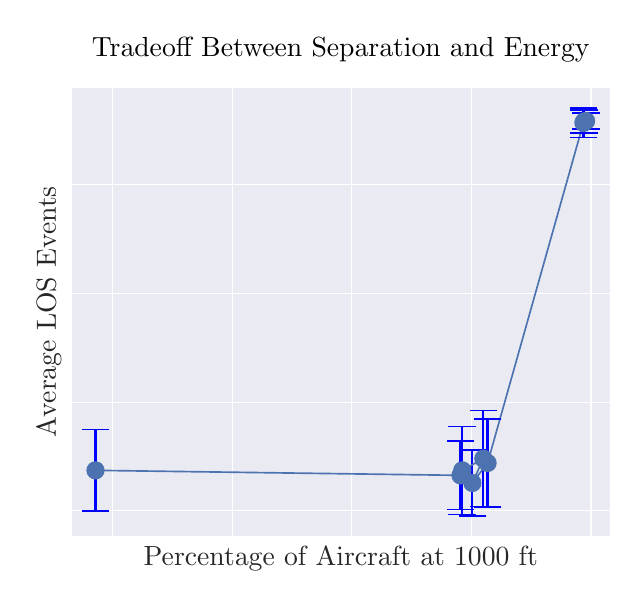
\begin{tikzpicture}

\definecolor{darkslategray38}{RGB}{38,38,38}
\definecolor{lavender234234242}{RGB}{234,234,242}
\definecolor{steelblue76114176}{RGB}{76,114,176}

\begin{axis}[
axis background/.style={fill=lavender234234242},
axis line style={white},
tick align=outside,
title={Tradeoff Between Separation and Energy},
x grid style={white},
xlabel=\textcolor{darkslategray38}{Percentage of Aircraft at 1000 ft},
xmajorgrids,
xmajorticks=false,
xmin=0.130367579600399, xmax=1.03286180003621,
xtick style={color=darkslategray38},
y grid style={white},
ylabel=\textcolor{darkslategray38}{Average LOS Events},
ymajorgrids,
ymajorticks=false,
ymin=-1.16772603652664, ymax=19.4513214113008,
ytick style={color=darkslategray38}
]
\path [draw=blue, thick]
(axis cs:0.171390044165663,-0.0162729012593024)
--(axis cs:0.171390044165663,3.7362729012593);

\path [draw=blue, thick]
(axis cs:0.781851972624718,0.0573907033213874)
--(axis cs:0.781851972624718,3.20260929667861);

\path [draw=blue, thick]
(axis cs:0.784742534521461,-0.164944443682345)
--(axis cs:0.784742534521461,3.88494444368235);

\path [draw=blue, thick]
(axis cs:0.820026311373226,0.190927796562548)
--(axis cs:0.820026311373226,4.60907220343745);

\path [draw=blue, thick]
(axis cs:0.801623614391582,-0.230496607079937)
--(axis cs:0.801623614391582,2.79049660707994);

\path [draw=blue, thick]
(axis cs:0.827098256656177,0.190024875775822)
--(axis cs:0.827098256656177,4.20997512422418);

\path [draw=blue, thick]
(axis cs:0.987379332685455,17.1659080181459)
--(axis cs:0.987379332685455,18.5140919818541);

\path [draw=blue, thick]
(axis cs:0.988390057391869,17.3803847577293)
--(axis cs:0.988390057391869,18.4196152422707);

\path [draw=blue, thick]
(axis cs:0.991839335470947,17.5574176840924)
--(axis cs:0.991839335470947,18.2997251730505);

\addplot [semithick, blue, mark=-, mark size=5, mark options={solid}, only marks]
table {%
0.171390044165663 -0.0162729012593024
0.781851972624718 0.0573907033213874
0.784742534521461 -0.164944443682345
0.820026311373226 0.190927796562548
0.801623614391582 -0.230496607079937
0.827098256656177 0.190024875775822
0.987379332685455 17.1659080181459
0.988390057391869 17.3803847577293
0.991839335470947 17.5574176840924
};
\addplot [semithick, blue, mark=-, mark size=5, mark options={solid}, only marks]
table {%
0.171390044165663 3.7362729012593
0.781851972624718 3.20260929667861
0.784742534521461 3.88494444368235
0.820026311373226 4.60907220343745
0.801623614391582 2.79049660707994
0.827098256656177 4.20997512422418
0.987379332685455 18.5140919818541
0.988390057391869 18.4196152422707
0.991839335470947 18.2997251730505
};
\addplot [semithick, steelblue76114176, mark=*, mark size=3, mark options={solid}]
table {%
0.171390044165663 1.86
0.781851972624718 1.63
0.784742534521461 1.86
0.820026311373226 2.4
0.801623614391582 1.28
0.827098256656177 2.2
0.987379332685455 17.84
0.988390057391869 17.9
0.991839335470947 17.9285714285714
};
\end{axis}

\end{tikzpicture}
